\documentclass[../Head/Main.tex]{subfiles}
\begin{document}
\section{Results}
The counted number of pumpkins were 21357, however this number can not be used. Two problems arose when counting the pumpkins:
\begin{itemize}
\item Part of the background is frequently counted as pumpkins
\item Some pumpkins are not counted
\end{itemize}
An example part of the orthomosaic with the counted pumpkins marked is seen in figure \ref{fig:counted_wrong}

\begin{figure}[H]
	\centering
	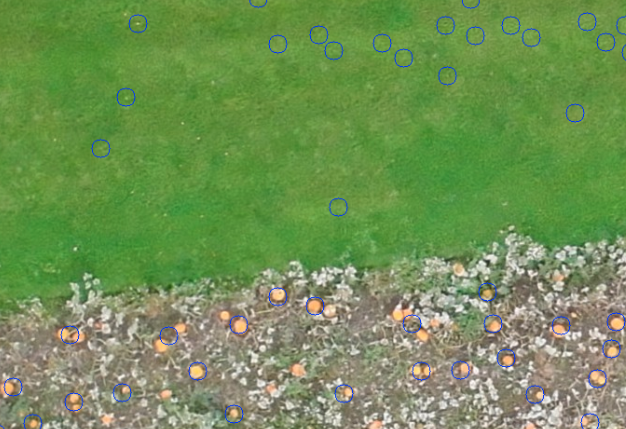
\includegraphics[scale=0.42]{../Figures/counted_wrong.png}
	\caption{Part of the orthomosaic with the counted pumpkins marked.}
	\label{fig:counted_wrong}
\end{figure}

It can be seen "pumpkins" are marked several places on the grass while several actual pumpkins were not counted.\par
The reason for this is the difference in color characteristics and illumination between the orthomosaic and the image that the pumpkin counting method was originally developed for. Part of the image used for the original color analysis is seen in figure \ref{fig:orig_img}.

\begin{figure}[H]
	\centering
	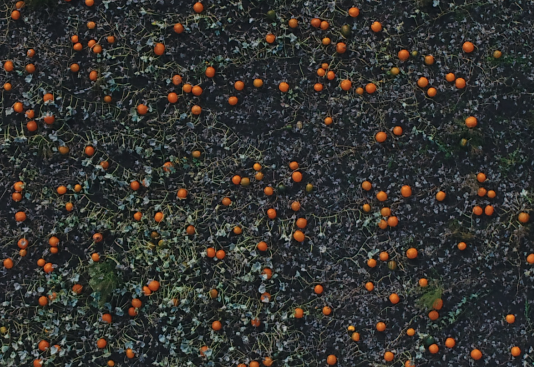
\includegraphics[scale=0.5]{../Figures/orig_image.png}
	\caption{Original image used for color analysis}
	\label{fig:orig_img}
\end{figure}

In comparison, part of the resulting orthomosaic is seen in figure \ref{fig:new_img}.

\begin{figure}[H]
	\centering
	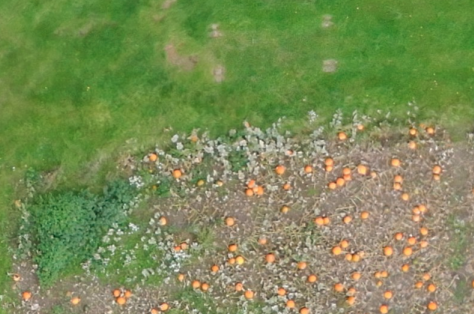
\includegraphics[scale=0.6]{../Figures/new_img.png}
	\caption{Part of the orthomosaic}
	\label{fig:new_img}
\end{figure}

It is clear that the color characteristics are quite different. The color spectrum of the pumpkins to be included in the segmentation is different than for the original image, the color spectrum of the green background is different than for the original image, and a new background color (the earth) is present in the orthomosaic.\par
A potential solution could be to perform a complete color analysis as originally done in the previous project. In the previous project, histograms for each color channel for the entire image was compared with the histograms of each channel for the pumpkins only. The result was a range of RGB values that would seperate the pumpkins from the background as well as possible. Similarly, the histograms of the pumpkins, the grass background, and the earth background could be inspected in order to find appropriate ranges of RGB values for segmenting the pumpkins in the orthomosaic. Due to time constraints, this was not implemented.

\section{Conclusion}
CONCLUSION ABOUT PHOTOGRAMMETRY STUFF HERE!?!?.\\

A large image handling procedure was implemented to divide the orthomosaic into tiles and expose each tile iteratively without keeping the entire orthomosaic in RAM.\\
A class \textit{PumpkinCounterOrthomosaic} was implemented that using the \textit{ImageDivisor} class and the \textit{PumpkinCounter} class counted the pumpkins for each tile in the orthomosaic. The overlapping counted pumpkins were then removed following an algorithm that across bordering tiles determined if the distance between pumpkin coordinates were within one pumpkin diameter.\\
Due to the completely different color spectrum of the orthomosaic compared to the image used for the original color analysis, the color segmentation were of no use for the orthomosaic. A new color analysis would have to be performed in order to obtain new values for segmentation of the images. Therefore, the resulting counted number of pumpkins is flawed. The new color analysis was not performed due to time constraints.
\end{document}